\chapter{Pr\'eliminaires -- Notions de base en \'electronique}

\section{Savoir lire un sch\'ema \'electronique}\label{sec:schematic}

Lire un sch\'ema \'electronique consiste à interpr\'eter un ensemble de symboles normalis\'es
qui repr\'esentent les composants, ainsi que leurs connexions entre eux.
Un sch\'ema ne montre pas l’agencement physique des composants sur une carte, mais leur
relation \'electrique. Comme le plan du m\'etro, les distances et angles ne sont pas
à l’\'echelle, mais les connexions sont correctes.

\subsection{Les symboles de base}

Chaque composant est repr\'esent\'e par un symbole normalis\'e, les symboles seront pr\'esent\'es
au fur et à mesure dans le document.
Voici quelques exemples de symboles courants :
\begin{itemize}
    \item \textbf{R\'esistance} :
    \raisebox{-0.5\height}{%
        \begin{circuitikz}
            \draw (0,0) to[R] (2,0);
        \end{circuitikz}
    }

    \item \textbf{Condensateur} :
    \raisebox{-0.5\height}{%
        \begin{circuitikz}
            \draw (0,0) to[C] (2,0);
        \end{circuitikz}
    }

    \item \textbf{Diode} :
    \raisebox{-0.5\height}{%
        \begin{circuitikz}
            \draw (0,0) to[D] (2,0);
        \end{circuitikz}
    }

    \item \textbf{Transistor NPN} :
    \raisebox{-0.5\height}{%
        \begin{circuitikz}
            \draw (0,0) to[short, o-o] (2,0);
            \draw (1,0) node[npn, anchor=B, rotate=0]{};
        \end{circuitikz}
    }

    \item \textbf{Source de tension} :
    \raisebox{-0.5\height}{%
        \begin{circuitikz}
            \draw (0,0) to[V] (2,0);
        \end{circuitikz}
    }

    \item \textbf{Source de courant} :
    \raisebox{-0.5\height}{%
        \begin{circuitikz}
            \draw (0,0) to[I] (2,0);
        \end{circuitikz}
    }

    \item \textbf{Masse} :
    \raisebox{-0.5\height}{%
        \begin{circuitikz}
            \draw (0,0) node[ground]{};
        \end{circuitikz}
    }

    \item \textbf{Op-amp} :
    \raisebox{-0.5\height}{%
        \begin{circuitikz}
            \draw (0,0) node[op amp, anchor=-] {};
        \end{circuitikz}
    }

    \item \textbf{Inductance} :
    \raisebox{-0.5\height}{%
        \begin{circuitikz}
            \draw (0,0) to[L] (2,0);
        \end{circuitikz}
    }

    \item \textbf{Interrupteur} :
    \raisebox{-0.5\height}{%
        \begin{circuitikz}
            \draw (0,0) to[spst] (2,0);
        \end{circuitikz}
    }
\end{itemize}

\subsection{Les connexions et nœuds}

Les fils reliant les symboles indiquent les conducteurs \'electriques.
Un point marqu\'e par un \textbf{nœud} (un petit rond noir) repr\'esente une connexion entre plusieurs fils.
En revanche, deux fils qui se croisent sans point ne sont pas connect\'es.

\begin{figure}[H]
  \centering
  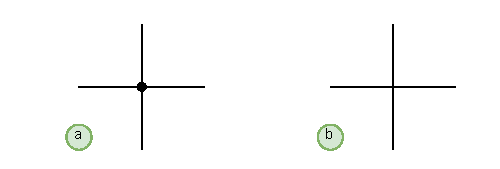
\includegraphics[width=0.8\textwidth]{wires.pdf}
  \caption{\fakecustommacro{a} : fils connect\'es avec un nœud. \fakecustommacro{b} : fils crois\'es sans connexion.}
\end{figure}


\subsection{Fl\'echage des tensions et des courants}
Pour analyser un circuit, il est souvent utile de fl\'echer les tensions et les courants.
\begin{itemize}
    \item \textbf{Tension} : La tension est une diff\'erence de potentiel entre deux points.
    On fl\`eche la tension de la borne positive (\(+\)) vers la borne n\'egative (\(-\)).
    \item \textbf{Courant} : Le courant est le flux de charges \'electriques.
    On fl\`eche le courant dans la direction du flux des charges positives (de \(+\) vers \(-\)).
\end{itemize}
Ces fl\`eches aident à visualiser comment l’\'energie circule dans le circuit.

\subsection{Exemple simple}

\begin{figure}[H]
    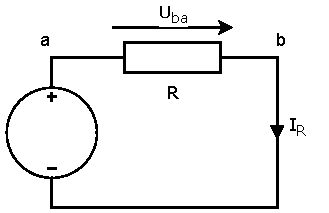
\includegraphics[width=0.7\textwidth]{example-schema.pdf}
    \caption{
        Un sch\'ema de maille simple avec une source de tension et une r\'esistance
    }
\end{figure}

\subsection{La lecture d’un circuit}

\begin{Note}
Pour lire un sch\'ema, on suit g\'en\'eralement ces \'etapes :
\begin{enumerate}
  \item Identifier la source d’\'energie (pile, alimentation).
  \item Rep\'erer la masse (r\'ef\'erence commune du circuit), si elle est pr\'esente.
  \item Suivre le parcours du courant à travers les composants.
  \item Reconna\^itre les sous-circuits classiques : diviseur de tension, filtre RC, pont redresseur, etc.
\end{enumerate}

Pour une analyse d'un circuit complexe, on peut ignorer les valeurs des composants et se concentrer sur la topologie du circuit,
c'est-à-dire rep\'erer comment les montages courants comme les redresseurs, amplificateurs, oscillateurs, etc. sont interconnect\'es.
\end{Note}

\section{Concepts \'electriques de base}
\subsection{R\'esistances}
La r\'esistance est un composant \'electronique qui \emph{limite le flux} de courant dans un circuit. Section d\'edi\'ee aux r\'esistances : \Cref{subsec:resistors}.

\subsection{R\'esistivit\'e}
La r\'esistivit\'e (\(\rho\)) est une propri\'et\'e physique des mat\'eriaux qui mesure leur \textbf{opposition} au passage du courant \'electrique. Elle est mesur\'ee en ohm-m\`etre (\unit{\ohm\meter}). La r\'esistivit\'e d\'epend de la nature du mat\'eriau, de sa temp\'erature, et de sa puret\'e. Les m\'etaux ont une r\'esistivit\'e faible, tandis que les isolants ont une r\'esistivit\'e \'elev\'ee. La r\'esistivit\'e est li\'ee à la r\'esistance (\(R\)) d’un conducteur par la formule~:
\[ R = \rho \dfrac{L}{A} \]
o\`u \(L\) est la longueur du conducteur et \(A\) sa section transversale.

\subsection{Conductivit\'e}
La conductivit\'e est une propri\'et\'e physique des mat\'eriaux qui mesure leur capacit\'e à conduire le courant \'electrique. Elle est d\'efinie comme l’inverse de la r\'esistivit\'e (\(\rho\)) et est mesur\'ee en siemens par m\`etre (\unit{\siemens\per\meter}). La conductivit\'e (\(\sigma\)) est donn\'ee par la formule :
\[\sigma = \dfrac{1}{\rho} \]
La conductivit\'e d\'epend de la nature du mat\'eriau, de sa temp\'erature, et de sa puret\'e. Les m\'etaux ont une conductivit\'e \'elev\'ee, tandis que les isolants ont une conductivit\'e faible. Voir \Cref{tab:conductivity} pour la conductivit\'e de quelques m\'etaux courants.
\begin{table}[h!]
    \centering
    \caption{Conductivit\'e \'electrique de quelques m\'etaux à \SI{20}{\unit{\celsius}}}
    \label{tab:conductivity}
    \begin{tabular}{l S[table-format=1.2e2]}
        \toprule
        \textbf{M\'etal} & \textbf{Conductivit\'e}~\unit{\siemens\per\meter} \\
        \hline
        Argent (Ag)      & 6.30e7 \\
        Cuivre (Cu)      & 5.96e7 \\
        Or (Au)          & 4.10e7 \\
        Aluminium (Al)   & 3.77e7 \\
        Magn\'esium (Mg)   & 2.30e7 \\
        Tungst\`ene (W)    & 1.89e7 \\
        Zinc (Zn)        & 1.69e7 \\
        Nickel (Ni)      & 1.43e7 \\
        Fer (Fe)         & 1.00e7 \\
        Plomb (Pb)       & 4.55e6 \\
        \'etain (Sn)       & 9.10e6 \\
        \bottomrule
    \end{tabular}
\end{table}

\subsection{Conductance}
La conductance (not\'ee \(G\)) est la grandeur qui mesure la \emph{facilit\'e} avec laquelle un courant \'electrique peut traverser un composant ou un circuit. C’est l’inverse de la r\'esistance (\(R\))~:
\[ G = \frac{1}{R} \]
L’unit\'e de la conductance est le \textbf{siemens} (\unit{\siemens}), anciennement appel\'e \textbf{mho} (\unit{\mho}), qui est l’inverse de l’ohm (\unit{\ohm}). Une conductance \'elev\'ee indique qu’un composant laisse facilement passer le courant, tandis qu’une conductance faible indique une opposition plus grande au passage du courant.

\subsection{Imp\'edance}
L'\textbf{imp\'edance} (not\'ee $Z$) g\'en\'eralise la notion de r\'esistance au r\'egime sinusoïdal. C’est une \emph{grandeur complexe} qui relie la tension et le courant~:
\[
Z = \frac{U}{I}
\]
On l’\'ecrit~:
\[
Z = R + jX
\]
o\`u~:
\begin{itemize}
  \item $R$ : r\'esistance (part r\'eelle)
  \item $X$ : r\'eactance (part imaginaire)
\end{itemize}
L’unit\'e de l’imp\'edance est l’\textbf{ohm} (\unit{\ohm}). Elle caract\'erise à la fois la dissipation (via $R$) et le stockage d’\'energie (via $X$) dans le circuit.

\subsection{Admittance}
L'\textbf{admittance} (not\'ee $Y$) est la \emph{grandeur inverse de l'imp\'edance}. Elle mesure la facilit\'e avec laquelle un courant traverse un circuit soumis à une tension alternative~:
\[
Y = \frac{1}{Z}
\]
C’est une grandeur complexe :
\[
Y = G + jB
\]
o\`u~:
\begin{itemize}
  \item $G$ : conductance (part r\'eelle, en siemens)
  \item $B$ : susceptance (part imaginaire, en siemens)
\end{itemize}

\subsection{Susceptance}
La \textbf{susceptance} (not\'ee $B$) repr\'esente la \emph{part imaginaire de l'admittance} d'un circuit.
Elle exprime la capacit\'e d'un composant à laisser passer le courant alternatif en raison de sa r\'eactance.
\[
B = \frac{1}{X}
\]
o\`u $X$ est la r\'eactance du composant (\unit{\ohm}).
L'unit\'e de la susceptance est le \textbf{siemens} (\unit{\siemens}).
\begin{itemize}
  \item Pour une \textbf{inductance} : $B_L = -\dfrac{1}{\omega L}$
  \item Pour une \textbf{capacit\'e} : $B_C = \omega C$
\end{itemize}

\subsection{R\'eactance}
La \textbf{r\'eactance} (not\'ee $X$) exprime la \emph{r\'esistance oppos\'ee au passage du courant alternatif} due à la pr\'esence d’une bobine ou d’un condensateur. Elle d\'epend de la fr\'equence $\omega = 2\pi f$~:
\[
X = \omega L \quad \text{(inductive)} \qquad \text{ou} \qquad X = -\frac{1}{\omega C} \quad \text{(capacitive)}
\]
Son unit\'e est l’\textbf{ohm} (\unit{\ohm}). Une r\'eactance positive est dite \textbf{inductive}, une r\'eactance n\'egative \textbf{capacitive}.
